\documentclass{standalone}
\usepackage{hsbcommon}
\usepackage{tikz}
\makeatletter\AtBeginDocument{\@buildstepset{1,2,3,4}}\makeatother
\usetikzlibrary{matrix,positioning}
\begin{document}
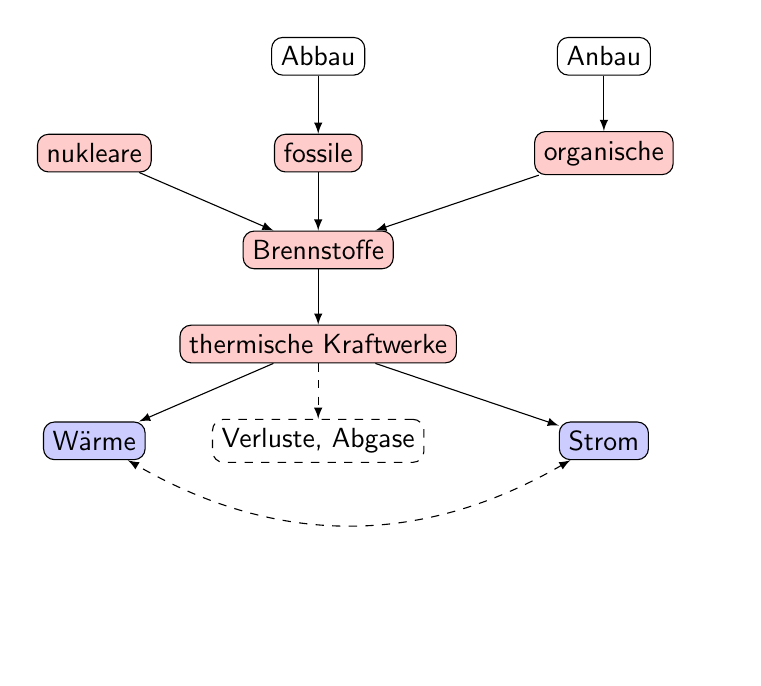
\begin{tikzpicture}[
    every node/.style={font=\sffamily},
    quelle/.style={draw,rounded corners},
    sink/.style={draw,dashed,rounded corners,fill=white},
        motor/.style={opacity=0},
        motorline/.style={opacity=0},
    fossil/.style={draw,rounded corners,fill=red!20},
        ee/.style={opacity=0},
        eeline/.style={opacity=0},
    produkt/.style={draw,rounded corners,fill=blue!20},
        kommentar/.style={draw=none},
    >=latex
]

\ifstep{2}{
    \tikzset{
        motor/.style={draw,dashed,rounded corners,fill=yellow!20},
        motorline/.style={draw},
    }
}

\ifstep{3}{
    \tikzset{
    ee/.style={draw,rounded corners,fill=green!20},
    eeline/.style={draw},
    }
}

\ifstep{4}{
    \tikzset{
    kommentar/.style={dashed}
    }
}


\matrix (m) [matrix of nodes, row sep=2em, column sep=1em, nodes={anchor=center},
] {
                & |[quelle]|Abbau                     & |[quelle]|Anbau         \\
    |[fossil]|nukleare    & |[fossil]|fossile                   & |[fossil]|organische    \\
                & |[fossil]|Brennstoffe               & |[motor]| Verbrennermotoren    \\
                & |[fossil]|thermische Kraftwerke     & |[motor]| Elektromotoren               \\
    |[produkt]|Wärme       & |[sink]|Verluste, Abgase                   & |[produkt]|Strom        \\
                &                           &  |[ee]|Erneuerbare KW     \\
    |[ee]|Sonne       & |[ee]|Wind                      & |[ee]|Wasser    \\
};

\draw[->] (m-1-2) -- (m-2-2);
\draw[->] (m-1-3) -- (m-2-3);

\draw[->] (m-2-1) -- (m-3-2);
\draw[->] (m-2-2) -- (m-3-2);
\draw[->] (m-2-3) -- (m-3-2);

\draw[->] (m-3-2) -- (m-4-2);

\draw[->,motorline] (m-3-2) -- (m-3-3);
\draw[->,motorline] (m-5-3) -- (m-4-3);

\draw[->] (m-4-2) -- (m-5-1);
\draw[->,dashed] (m-4-2) -- (m-5-2);
\draw[->] (m-4-2) -- (m-5-3);

\draw[->,eeline] (m-7-1) -- (m-6-3);
\draw[->,eeline] (m-7-2) -- (m-6-3);
\draw[->,eeline] (m-7-3) -- (m-6-3);

\draw[->,eeline] (m-6-3) -- (m-5-3);

\draw[->,eeline,kommentar] (m-7-1) -- (m-5-1);

\draw[<->,dashed,bend left=30] (m-5-3) to (m-5-1);


\end{tikzpicture}
\end{document}